\documentclass[a4paper]{article}

\usepackage[utf8]{inputenc}
\usepackage[spanish]{babel}
\usepackage{graphics}
\usepackage{caption}
\usepackage{subcaption}
\usepackage[demo]{graphicx}
\usepackage{enumitem}
\usepackage{longtable}
\usepackage{listings}
\usepackage{listingsutf8}
\usepackage{framed}
\usepackage{float}
\usepackage{hyperref}

\begin{document}

\title{Informe del sistema de recuperación tradicional MiniTREC}
\author{
	Jaime Ruiz-Borau Vizárraga\\
	\texttt{546751}
	\and
	Alberto Sabater Bailón\\
	\texttt{546297}
	}
\date{}
\maketitle

\section{Arquitectura del software desarrollado}
\paragraph{}El siguiente diagrama de clases representa el diseño arquitectural del software desarrollado para el sistema de recuperación tradicional:
\begin{figure}[!hb]
	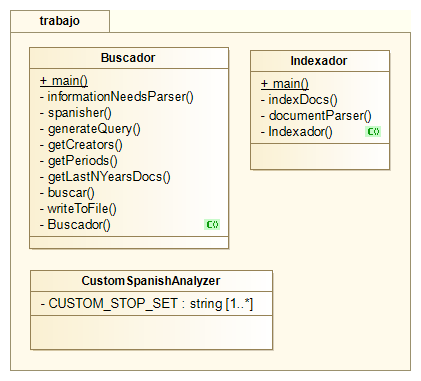
\includegraphics[width=\linewidth]{DiagramClass.png}
	\caption{Diagrama de clases y paquetes del sistema}
	\label{fig:class}
\end{figure}
\\
\newpage
\paragraph{}Como se puede apreciar en el diagrama, todas las clases se alojan en el paquete \textbf{trabajo}. Los nombres de las principales clases se explican por sí mismos: la clase \textit{Indexador} es la que posee métodos para indexar una colección de documentos especificada por parámetro tal y como solicita el enunciado; y la clase \textit{Buscador} es la que se encarga de realizar las consultas de las necesidades de información en base al índice creado por la clase Indexador.
\paragraph{}Adicionalmente existe una tercera clase, \textit{CustomSpanishAnalyzer}, que extiende a la clase de Lucene \textbf{Analyzer}. Reimplementa el método \textit{createComponents}, que permite modificar las StopWords que suprimirá el analizador a la hora de lematizar una consulta.
\\
\newline Como detalle adicional, ambas clases Buscador e Indexador poseen un booleano \textbf{DEBUG} que a no ser que sea establecido manualmente a \textbf{true} impedirá que ambos programas muestren salida alguna por pantalla.

\section{Técnicas empleadas}
\subsection{Técnicas empleadas en Indexador}
\paragraph{}Dada la naturaleza de la colección de documentos del Zaguán, se ha optado por realizar un análisis de las etiquetas de los documentos extrayendo la información de todas ellas siguiendo el estándar de la iniciativa Open Archives \textbf{(Open Archives Initiate)}. Dicho estándar establece una serie de etiquetas en documentos XML: \textbf{Title} \textit{(título)}, \textbf{Creator} \textit{(autor)}, \textbf{Subject} \textit{(materia)}, \textbf{Description} \textit{(descripción)}, \textbf{Publisher} \textit{(editor)}, \textbf{Contributor} \textit{(asistente)}, \textbf{Date} \textit{(fecha)},
\textbf{Type} \textit{(tipo)}, \textbf{Format} \textit{(formato)}, \textbf{Identifier} \textit{(identificador)}, \textbf{Source} \textit{(fuente)}, \textbf{Language} \textit{(idioma)}, \textbf{Relation} \textit{(relacion)}, \textbf{Coverage} \textit{(cobertura)} y \textbf{Rights} \textit{(derechos)}.
\paragraph{}Aunque varios de ellos no aparecen en la colección de documentos del Zaguán, se implementaron igualmente su análisis y extracción en el caso de que en el futuro se llegasen a incluir dichas etiquetas en los documentos del Zaguán (mayor modularidad futura).
\paragraph{}Para cada etiqueta descrita anteriormente, simplemente se crearon los campos asociados con el mismo nombre y lo siguientes tipos:
\begin{itemize}
	\item \textbf{TextField} - Title, Creator, Subject, Description, Publisher y Contributor
	\item \textbf{IntField} - Date
	\item \textbf{StringField} - Type, Format, Identifier, Source, Language, Relation, Coverage y Rights
\end{itemize}
\paragraph{}Además de este análisis y extracción de las etiquetas, Indexador no emplea el típico Analyzer de Lucene, emplea el \textbf{CustomSpanishAnalyzer} que se mencionó en el diagrama de clases y que se explica en el apartado que describe las técnicas empleadas en la clase Buscador.
\\
\newpage
\subsection{Técnicas empleadas en Buscador}
\paragraph{}Para la clase Buscador, se han empleado las siguientes técnicas y metodologías a la hora de realizar una consulta en base a una necesidad de información:
\begin{itemize}
	\item \textbf{Correcto espaciado de la necesidad de información}:
	\\ Tal y como se proporcionó el fichero XML de necesidades de información, existían saltos de línea y tabuladores innecesarios que se optó por suprimir antes de procesar la necesidad para convertirla en consulta. 
	\paragraph{}Asimismo, sabiendo que el analizador de Lucene toma por distintos tokens la misma palabra seguida de un punto que sin el punto (para Lucene son diferentes tokens los términos 'agua' y 'agua.'), también se optó por suprimir de la necesidad inicial todos los puntos.
	\item \textbf{Lematización de la consulta}:
	\\ Utilizando el CustomSpanishAnalyzer mencionado anteriormente, toda la necesidad de información queda lematizada a las raíces más importantes de cada palabra, suprimiendo palabras innecesarias (StopWords). 
	\paragraph{}Concretamente, el CustomSpanishAnalyzer diseñado, hereda las StopWords del \textbf{SpanishAnalyzer} por defecto de Lucene, y añade las siguientes: \textit{'interes', 'trabaj', 'llam', 'relacion', 'cuy', 'llam', 'period', 'gust', 'sab', 'articul', 'relacionad', 'hech', 'englob', 'tesis', 'trat', 'quier', 'document', 'encontr', 'situ', 'element', 'pertenezc'} y \textit{'mund'}.
	\paragraph{}Estas StopWords personalizadas fueron resultado de analizar individualmente cada consulta y eliminar las lematizaciones que se consideraron innecesarias para la consulta.
	\item \textbf{Pre-procesamiento de la necesidad de información}:
	\\Tras la lematización, se implementaron las siguientes técnicas antes de que el buscador procesase la consulta de forma general:
	\\
	\newline \textbf{1.-Búsqueda de autores en la necesidad:} Si el usuario en su necesidad de información especificó la palabra 'autor' y ésta, en algún momento de la misma necesidad, venía seguida de alguna otra palabra que comenzase por mayúscula, esta técnica asumiría que dicha palabra al comenzar por letra mayúscula es el \textbf{nombre del autor} del que se buscan documentos.
	\paragraph{}Por tanto, tras obtener el nombre del autor de los documentos que se buscan, se añadiría a la consulta final (de ahora en adelante \textbf{query}) una consecucion de TermQuerys (un tipo concreto de Querys en Lucene para términos) que \textbf{buscarán que haya coincidencias en el campo 'creator' para dicho nombre de autor}.
	Una vez hecho esto, se quita de la consulta lematizada final los términos autor y los nombres propios considerados.
	\\
	\newpage\textbf{2.-Búsqueda de períodos de años:} En ocasiones, el usuario especifica en su necesidad de información un período de años que buscar, bien sea el período de años entre los que pretende encontrar un trabajo o un período de años histórico sobre los que pretende encontrar un trabajo que hable de ellos.
	\paragraph{}Por ende, se ha implementado en la clase Buscador que busque en la consulta lematizada números de 4 cifras consecutivos y los considere un período de tiempo, de tal forma que a la query final se le añadirán unas \textbf{RangeQuerys} (querys para la comprobación de un rango de números sobre campos) sobre el campo \textbf{date} si dicho período de años es mayor o igual a 2008, fecha a partir de la cual existen documentos en el Zaguán. De esta forma la consulta se reducirá a documentos que se hallen dentro de dicho período especificado.
	\paragraph{}Para el resto de períodos, no se añaden querys de ningún tipo en particular, puesto que al final lo que queda de la consulta lematizada se especificará que se busque en los campos \textbf{description} y \textbf{title}. Se retirarán de la consulta lematizada los períodos de tiempo que sean mayores de 2008.
	\\
	\newline \textbf{3.-Búsqueda de la expresión 'últimos n años':} Como caso particular de las necesidades de información especificadas, se ha tomado en consideración el caso de que el usuario especifique en su necesidad de información que desea encontrar documentos cuya fecha de creación se halle entre los últimos n años.
	\\ 
	\newline Es por ello que se ha decidido buscar en la necesidad lematizada los términos 'últimos', un entero (n) y 'años', tras lo cual sabiendo el entero n y el año actual se puede generar una \textbf{RangeQuery} sobre el campo \textbf{date} que restringa los documentos cuya creación no esté comprendida en el rango descrito. Si se encuentran dichos términos, se retirarán de la consulta lematizada final.
	\\
	\newline \textbf{4.-Procesamiento de la consulta lematizada final:} Finalmente, tras todo el procesamiento expuesto anteriormente, la consulta lematizada restante es procesada de manera estándar. Se generarán TermQuerys para cada término que quede en la lista y se buscarán tanto en los campos \textbf{title} como \textbf{description}.
\end{itemize}
\newpage
\subsection{Algoritmo empleado para el ranking}
\paragraph{}El algoritmo utilizado para el cálculo del ranking, es el que utiliza Lucene por defecto. Dicho algoritmo usa una combinación del modelo de \textbf{espacio vectorial (VSM) y el modelo booleano} para determinar lo relevante que es un fichero.
\paragraph{}La idea general es que cuanto más veces aparece cada término de una query en un documento respecto del número de veces que ese término aparece en el resto de documentos de la colección, más relevante es ese documento para esa query.
Usa el modelo booleano para reducir el número de documentos devueltos haciendo uso de la lógica booleana en la specificación de la query.
\section{Resultados obtenidos}

\section{Otros puntos}

\end{document}